\section{Course Overview}

ME 513: Thermodynamics is a lecture based class that focuses on the interplay of heat, work, and energy in both
open and closed loop systems. While there is no lab portion to the class, significant lecture time is spent
solving problems and working examples, and a new homework is assigned every lecture to give students a chance
to apply the new concepts taught that day.

Most problems in thermodynamics follow a similar solution path. First, students must recognize the different
states in the system. Once the different states are identified, the values for temperature, power, energy,
entropy, etc. must be found for each state. The exact values needed, and retrievable, vary depending on the
given system. This process is known as setting the state. Once the state has been set, known laws of
thermodynamics can be applied and the question can be solved.

For most questions, the majority of time is spent setting the state. This involves using known properties, 
usually given in the problem statement, to look up values in property tables in a thermodynamics textbook. 
This often proves to be a very time consuming process, especially when interpolation is required to get 
property values. And once iteration is introduced, such as in a design problem, manually searching through
tables becomes impractical, if not impossible. This is where the use of a programming language would become 
highly beneficial.

Thermodynamics, as it currently stands, make no use of programming to complete assignments.
This can be attributed to ME 513 coming prior to ME 400, the only programming class in the 
curriculum. However, with the recent programming additions made to DEN 161, students have been introduced
to programming and, with the help of an example, should be capable of solving these questions as a small
project or assignment.

\section{New Assignments}

Since no assignments currently make use of programming, two new asssignments have been created to demonstrate
how programming could be beneficial to the course. Both assignments will make use of a Python library called
PYroMat, a free, open source library dedicated to making thermodynamic properties readily available.
They will also both make use of Jupyter Notebooks for cleanly presenting questions, commentaries, and code
while solving the question.

The first assignment, Assignment \ref{thermo_assignment_1}, is a five state system that does not require 
iteration or plotting. It follows the structure of a typical question in thermodynamics well. The student 
must identify the states, list the known properties for each state, and then either search for additional 
values in a table or calculate them with known values. After this, the laws of thermodynamics are applied, 
equations are balanced, and the questionis solved.

\assignments{ME 513: Assignment 1}
\label{thermo_assignment_1}

\begin{tcolorbox}[breakable, enhanced jigsaw, title=ME 513: Assignment \ref{thermo_assignment_1}, 
    colframe=blue!70!white, colback=gray!20]

    \textbf{Problem Statement}

    Water is the working fluid in a Rankine cycle. Steam exits the steam generator at 1500 
    lbf/in\textsuperscript{2}  and 1100°F. Due to heat transfer and frictional effects in 
    the line connecting the steam generator and turbine, the pressure and temperature at the 
    turbine inlet are reduced to 1400 lbf/in\textsuperscript{2} and 1000°F, respectively. Both the 
    turbine and pump have isentropic efficiencies of 85\%. Pressure at the condenser inlet 
    is 2 lbf/in\textsuperscript{2}, but due to frictional effects the condensate exits the 
    condenser at a pressure of 1.5 lbf/in\textsuperscript{2} and a temperature of 110°F. The 
    condensate is pumped to 1600 lbf/in\textsuperscript{2} before entering the steam generator. 
    The net power output of the cycle is 1x10\textsuperscript{9} Btu/h. Cooling water experiences 
    a temperature increase from 60°F to 76°F, with negligible pressure drop, as it passes 
    through the condenser. Determine for the cycle:

    \begin{enumerate}
        \item the mass flow rate of steam, in lb/h.
        \item the rate of heat transfer, in Btu/h, to the working fluid passing through the steam 
        generator. 
        \item the thermal efficiency.
        \item the mass flow rate of cooling water, in lb/h.
    \end{enumerate}

    Be sure to leave specify all assumptions and comment on the functionality of the code. 
    To access the thermodynamic tables for water, import PYroMat using the cell below.

    \tcblower
    \textbf{Problem Solution}

    For the full solution, see Appendix \ref{appendix:appendix_github}. Below is an example of 
    importing PYroMat, setting the correct units, and accessing property data.

    \begin{python}
    import pyromat

    pyromat.config["unit_energy"] = "BTU"
    pyromat.config["unit_force"] = "lbf"
    pyromat.config["unit_length"] = "in"
    pyromat.config["unit_mass"] = "lb"
    pyromat.config["unit_matter"] = "lb"
    pyromat.config["unit_molar"] = "lbmol"
    pyromat.config["unit_pressure"] = "psi"
    pyromat.config["unit_temperature"] = "F"
    pyromat.config["unit_volume"] = "ft3"
    H2O = pyromat.get("mp.H2O")

    # State 1
    p1 = 1400 # lbf/in^2
    T1 = 1000 # deg F
    n1 = 0.85 # dimensionless
    h1 = H2O.h(T=T1, p=p1) # Btu/lb
    s1 = H2O.s(T=T1, p=p1) # Btu/(lb*F)
    \end{python}
\end{tcolorbox}

The second assignment, Assignment \ref{thermo_assignment_2}, better showcases the benefits of 
programming. This question uses both iteration and plotting to show the changes in quality 
and thermal efficiency as the pressure increases. If done by hand, this would be a difficult 
and tedious task. But when programming, it only requires a few extra lines of code.

\assignments{ME 513: Assignment 2}
\label{thermo_assignment_2}

\begin{tcolorbox}[breakable, enhanced jigsaw, title=ME 513: Assignment \ref{thermo_assignment_2}, 
    colframe=blue!70!white, colback=gray!20]

    \textbf{Problem Statement}

    Steam heated at constant pressure in a steam generator enters the first stage of a
    supercritical reheat cycle at 28 MPa, 520°C. Steam exiting the first-stage turbine at 6 MPa is
    reheated at constant pressure to 500°C. Each turbine stage has an isentropic efficiency of 78%
    while the pump has an isentropic efficiency of 82\%. Saturated liquid exits the condenser that
    operates at constant pressure, p.

    \begin{enumerate}
        \item For p = 6 kPa, determine the quality of the steam exiting the second stage of the 
        turbine and the thermal efficiency.
        \item Plot the quantities of part (1) versus p ranging from 4 kPa to 70 kPa.
    \end{enumerate}

    Be sure to leave specify all assumptions and comment on the functionality of the code. 

    \tcblower
    \textbf{Problem Solution}

    For the full solution, see Appendix \ref{appendix:appendix_github}. Below is an example of 
    iterating through varying pressure values and plotting the result

    \begin{python}
    p_list = [x * 10**(-3) for x in range(4, 71)]
    x_list = []
    n_list = []

    for p in p_list:
        # State 4
        p4 = p # MPa
        x4s = H2O.T(s=s3, p=p4, quality=True)[1]
        h4s = H2O.h(p=p4, x=x4s)
        h4 = h3 - nt2 * (h3 - h4s)

        # State 5
        p5 = p # MPa
        h5 = H2O.h(p=p5, x=0)
        v5 = H2O.v(p=p5, x=0)

        # State 6
        h6 = h5 + 1000 * v5 * (p6 - p5) / (np1)

        # Find the quality of the steam
        hf4 = H2O.h(p=p4, x=0)
        hfg4 = H2O.h(p=p4, x=1) - H2O.h(p=p4, x=0)
        x4 = (h4 - hf4) / hfg4
        x_list.append(x4)

        # Find the thermal efficiency of the cycle
        n = ((h1-h2)+(h3-h4)-(h6-h5))/((h1-h6)+(h3-h2))
        n_list.append(n)

    plt.figure()
    plt.plot(p_list, x_list)
    plt.title("Quality vs Condenser Pressure")
    plt.xlabel("Pressure (MPa)")
    plt.ylabel("Quality (unitless)")
    plt.show()
    \end{python}
    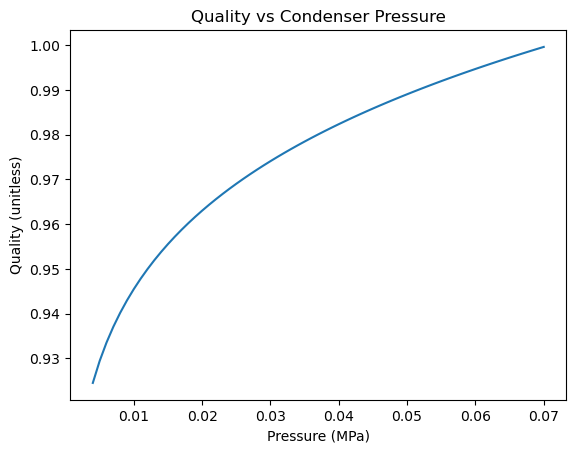
\includegraphics[width=\textwidth]{thermo_assignment_2.png}
\end{tcolorbox}

Using programming in this manner gives students a better idea of how real problems are solved by introducing
them to a more efficient and powerful solution method. These questions would also directly correlate to Abet 
Student Outcomes 1, 6, and 7 and weakly correlate to Outcome 3, as seen in Appendix \ref{appendix:appendix_abet}.

\section{Project Deliverables}

In the GitHub repository associated with this paper, which can be found in Appendix \ref{appendix:appendix_github},
the folder titled ``thermodynamics'' contains both the problem statements and solution guides for the two questions
introduced in the previous section. The folder also contains a README that details what is in each file and 
what software is needed to complete the assignments. 

For these projects to be added to the class, the instructor would simply need to give the skeleton files to 
students as a problem statement. It may be beneficial to use question 8.23 as an in-class example both to serve 
as a reminder of how to use Python with Jupyter Notebooks as well as a demonstration of how to use PYroMat to 
access material properties and change property units.
